% JKAIA 2026 (2026 한국인공지능학회 추계학술대회) -- General (Poster) track
% Template: kaia.cls (downloaded 2026-10-15 from the 논문제출 안내 page; 10pt, A4).
% Poster-track rule: a 1--2 page summary built from this template with title, authors, affiliations,
% abstract (optional). Review is single-blind, so author names stay in the PDF. Paper in English;
% the EasyChair abstract field is filled in Korean.
%
% Workflow: main_ko.tex is the Korean WORKING COPY with the same paragraph structure. The author edits
% the Korean text; the same edits are then applied here, paragraph by paragraph. This file is the SUBMISSION.
%
% Build:  tectonic -X compile main.tex   (or pdflatex main; bibtex not needed)
%
% Notes on the template:
%  * kaia.cls \maketitle switches to \twocolumn[...]; the official sample then draws a full-width
%    \fbox{\parbox{\textwidth}{...}} over both columns, which cannot break across pages. For a
%    two-page summary we keep the page one-column and draw the frame with mdframed (page-breakable).
%  * kaia.cls asks for Times via times/mathptmx. Under XeTeX (tectonic) those fonts are not mapped,
%    so we load the system Times New Roman; pdflatex/Overleaf keep the class default.

\documentclass[nouppercase]{kaia}
\usepackage{amsmath}
\usepackage{booktabs}
\usepackage{graphicx}
\usepackage[framemethod=TikZ]{mdframed}
\usepackage{iftex}
\ifXeTeX
  \usepackage{fontspec}
  \setmainfont{Times New Roman}
\fi
\usepackage{multicol}
\makeatletter
\newenvironment{posterrefs}{\par\vspace{2pt}\noindent{\small\textbf{References}}\par
  \def\@openbib@code{\scriptsize\setlength{\itemsep}{0pt}\setlength{\parsep}{0pt}\setlength{\topsep}{0pt}}%
  \let\section\@gobbletwo
  \setlength{\multicolsep}{0pt}\vspace{-0.8\baselineskip}%
  \begin{multicols}{2}\begin{thebibliography}{7}}{\end{thebibliography}\end{multicols}}
\makeatother
\AtBeginDocument{\hypersetup{pdftitle={Imagine Once, Act Fast: Lightweight Action Readout from a Frozen Driving World-Action Model},pdfauthor={YongHwi Song, Hyunsoo Kang}}}
\graphicspath{{../figures/}}
\expandafter\def\expandafter\UrlBreaks\expandafter{\UrlBreaks\do\-}  % allow URL line breaks at hyphens

\makeatletter
\renewcommand{\twocolumn}[1][]{#1}   % keep one column; \maketitle's optional argument is still typeset
\makeatother
\mdfsetup{linewidth=0.4pt, linecolor=black, innerleftmargin=7pt, innerrightmargin=7pt,
          innertopmargin=4pt, innerbottommargin=4pt, skipabove=4pt, skipbelow=4pt}

\title{Imagine Once, Act Fast: Lightweight Action Readout from a Frozen Driving World-Action Model}

\author{YongHwi Song}{a}
\author{Hyunsoo Kang}{a}
\affiliation{School of Information and Communication Engineering, Chungbuk National University, Cheongju, Republic of Korea, \{thddydgnl1937@gmail.com, hskang@chungbuk.ac.kr\}}{a}

\begin{document}

\maketitle
\vspace{-28pt}

\begin{mdframed}

\begin{abstract}
Driving world-action models (WAMs) such as DriveWAM imagine future video latents with a 5B video diffusion transformer and then run the same backbone ten more times to denoise a 4-second action chunk, the largest latency term in the pipeline. We ask whether a small head can read the trajectory from the frozen backbone right after its first future-denoising pass (future pass 1). We hook three transformer blocks at that pass, regress the trajectory with a 10M-parameter state-fusion head (SF3) and stop inference there; the official checkpoints are never updated. On NAVSIM it is 4.2 times faster than official DriveWAM and 2.2 times faster than the fastest quality-preserving reduced-step baseline, at a cost of 0.2 to 0.4 PDMS. On the NVIDIA PhysicalAI-AV official test it is 11.8 times faster with trajectory error comparable to DriveWAM: lower than its official single sample and, on the dev set, on par in ADE with the mean of four samples and about 0.1 m higher in FDE. Future pass 1 already carries most of the action information, further denoising brings no significant gain, and more head-training data steadily closes the gap.
\end{abstract}
\begin{keywords}
World-action model, autonomous driving, efficient inference, video diffusion, trajectory planning
\end{keywords}

\subsection{Problem Setup}
DriveWAM~\cite{shi2026drivewam} (6.24B parameters, built on Wan2.2-TI2V-5B~\cite{wan2025wan}) is an autoregressive video-action policy: conditioned on past frames, the ego state and a guidance sentence, it denoises future video latents in three passes of the diffusion transformer and then a 4-second action chunk in ten more passes of the same transformer (B10). Without retraining the backbone, we ask at which point of the future generation, and from which depth, the action can be read out in a single pass. Quality is compared with B10 and with $B^{*}$, the fastest reduced-step variant that matches B10 quality on a development (dev) set, since reducing steps needs no training.

\subsection{Novelty}
(1) \textit{Readout from a frozen WAM's own imagination.} Light-WAM~\cite{li2026lightwam} and Faster-WAM~\cite{ma2026fasterwam,zhao2026fasterwam} train or adapt the backbone with a light action expert. We keep the public DriveWAM checkpoints frozen, replace only the action generator, and read the backbone at future pass 1. Our contribution is where and when to read, not the head architecture. (2) \textit{Three readout phases}: \texttt{current}, \texttt{first} and \texttt{terminal} (Table~\ref{tab:diag}). (3) \textit{Pre-registered evaluation}: splits, $B^{*}$ selection, quality thresholds and the head were fixed before results were read, and the locked final sets were evaluated once. (4) \textit{Two evaluation pitfalls}: the public NAVSIM backbone has memorized its training scenes (B10 ADE 0.076 m on navtrain vs.\ 0.598 m on navtest), and the single-seed PhysicalAI protocol is seed-sensitive (B10 dev ADE 0.82--0.93 m).

\subsection{Algorithms}
\textbf{Frozen backbone and taps.} The official inference loop is re-implemented and verified bitwise against upstream; forward hooks read blocks 10, 20 and 30, and with \texttt{first} features inference exits right after future pass 1 (Fig.~\ref{fig:overview}).
\textbf{SF3 head} (9.98M parameters, 0.16\% of the backbone). The head adopts the multi-level state-fusion design of Light-WAM's action expert~\cite{li2026lightwam} (16 learned queries per block, a fusion MLP and per-step decoding). It differs in what it is attached to and what it predicts: it is trained alone on the frozen DriveWAM backbone, reads future pass 1 instead of the observation, takes the ego state, and predicts normalized displacement and heading per step (8 poses at 2 Hz on NAVSIM, 40 steps at 10 Hz on PhysicalAI). Training: 40 epochs, last checkpoint, no selection on evaluation data.
\textbf{Baselines and statistics.} B10 and the reduced-step variants B05- to B01-opt (5 to 1 action steps); $B^{*}$ is the fastest of them that matches B10 on the dev set. Cluster-paired bootstrap CIs; latency from interleaved runs on one RTX A5000.

\begin{center}
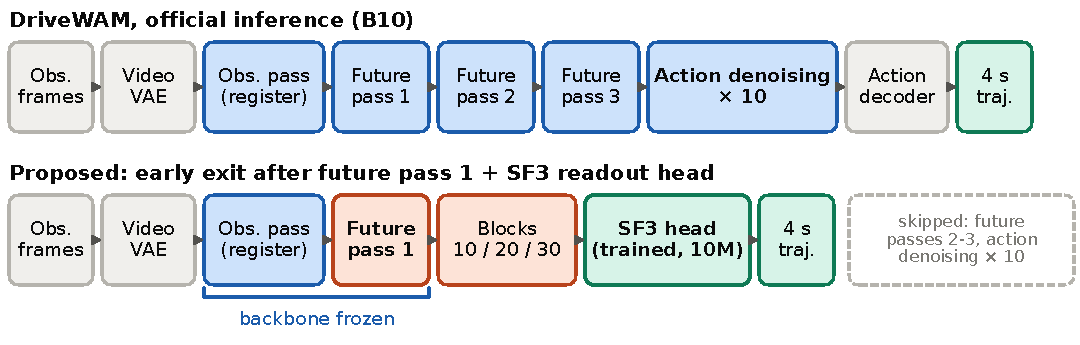
\includegraphics[width=0.68\linewidth]{fig_overview_poster.pdf}
\captionof{figure}{Official DriveWAM inference (top) and the proposed readout (bottom). The backbone is never updated.}
\label{fig:overview}
\end{center}

\subsection{Experiments}
\textbf{Setup.} NAVSIM v1.1~\cite{dauner2024navsim}: one scene $\rightarrow$ one 4-s trajectory, official PDMS; head trained on 92,599 navtrain scenes; navtest split by log into a dev set (3,250 scenes) and a locked final set (8,896 scenes). PhysicalAI-AV~\cite{nvidia2025physicalai}: one clip $\rightarrow$ five 4-s chunks with teacher forcing, official ADE/FDE; head trained on the public 20k clips, dev set = 1,000 val clips, final set = official test 1k.

\begin{center}
\small
\setlength{\tabcolsep}{5pt}
\begin{tabular}{lcc@{\hskip 14pt}ccc}
\toprule
 & \multicolumn{2}{c}{NAVSIM navtest-final} & \multicolumn{3}{c}{PhysicalAI-AV official test 1k} \\
\cmidrule(lr){2-3}\cmidrule(lr){4-6}
Model & PDMS $\uparrow$ & p50 (ms) $\downarrow$ & ADE (m) $\downarrow$ & FDE (m) $\downarrow$ & p50 (ms) $\downarrow$ \\
\midrule
DriveWAM B10 (official)      & 89.67 & 797.9 & 0.802 & 2.384 & 837.8 \\
$B^{*}$ (selected on dev) & 89.65 (B02-opt) & 420.7 & 0.842 (B03-opt) & 2.362 & 434.0 \\
SF3-first (ours), seed 17 & 89.25 & \textbf{189.0} & 0.750 & 2.244 & \textbf{70.9} \\
SF3-first (ours), seed 29 & 89.49 & \textbf{189.0} & 0.748 & 2.244 & \textbf{70.9} \\
SF3-first (ours), seed 43 & --    & --    & 0.762 & 2.287 & \textbf{70.9} \\
\bottomrule
\end{tabular}
\captionof{table}{Locked final sets, evaluated once. p50: median latency per decision on one RTX A5000; NAVSIM times the whole policy call, PhysicalAI the decision after history registration (128 dev clips). NAVSIM $\Delta$PDMS vs.\ B10: $-0.42\,[-0.76,-0.08]$ / $-0.17\,[-0.56,+0.27]$ (95\% CI).}
\label{tab:final}
\end{center}

\textbf{Outcome.} PhysicalAI: all seeds are below the official single-sample B10 in ADE ($-0.040$ to $-0.054$ m) and FDE ($-0.10$ to $-0.14$ m) at 6.1 times the speed of $B^{*}$. NAVSIM: 0.17 to 0.42 PDMS below B10 at 2.2 times the speed of $B^{*}$; collisions improve (NC +0.15 to +0.17) while drivable-area compliance drops (DAC $-0.35$ to $-0.51$).
\textbf{One future pass is enough} (Table~\ref{tab:diag}). \texttt{first} clearly beats \texttt{current} on both benchmarks, while \texttt{terminal} brings no significant gain over \texttt{first}. \textbf{More head-training data closes the gap}: the NAVSIM gap to B10 shrinks from $-4.2$ to $-0.4$ PDMS between 4k and 92.6k scenes.
\begin{center}
\footnotesize
\setlength{\tabcolsep}{6pt}
\begin{tabular}{lcc}
\toprule
Readout phase, head-train set & NAVSIM navtest-dev PDMS (seed 17 / 29) & PhysicalAI dev ADE (m, 3-seed mean) \\
\midrule
\texttt{current} (observation only), 4k & 83.20 / 83.61 & 0.926 \\
\texttt{first} (future pass 1), 4k & 86.60 / 86.89 & 0.813 \\
\texttt{terminal} (all future passes), 4k & 87.34 / 86.28 & 0.825 \\
\texttt{first}, 20k & 89.36 / 90.00 & 0.762 \\
\texttt{first}, 92.6k & 90.43 / 90.58 & -- \\
DriveWAM B10 (reference) & 90.93 & 0.821 \\
\bottomrule
\end{tabular}
\captionof{table}{Dev-set results by readout phase and head-training data. \texttt{first} vs.\ \texttt{current}: +3.3 PDMS, $-0.11$ m ADE (95\% CIs exclude 0).}
\label{tab:diag}
\end{center}

\textbf{Limitations.} Mean-error metrics favor a deterministic regressor, so we do not claim higher accuracy than DriveWAM: on the PhysicalAI dev set, against the mean of four B10 samples the readout is on par in ADE and about 0.1 m worse in FDE. The phase comparison uses 4k head-training data. Code: \url{github.com/thddydgnl/drivewam-lightweight-action-readout}.

\begin{posterrefs}
\bibitem{shi2026drivewam} C.~Shi et al., DriveWAM, arXiv:2605.28544, 2026.
\bibitem{wan2025wan} Team Wan, Wan: open and advanced large-scale video generative models, arXiv:2503.20314, 2025.
\bibitem{li2026lightwam} Z.~Li et al., Light-WAM, arXiv:2606.08242, 2026.
\bibitem{ma2026fasterwam} L.~Ma et al., Faster-WAM (deep action modules), arXiv:2608.02365, 2026.
\bibitem{zhao2026fasterwam} W.~Zhao et al., Faster-WAM (future conditioning), arXiv:2608.04404, 2026.
\bibitem{dauner2024navsim} D.~Dauner et al., NAVSIM, NeurIPS Datasets and Benchmarks, 2024.
\bibitem{nvidia2025physicalai} NVIDIA, PhysicalAI-Autonomous-Vehicles dataset, 2025.
\end{posterrefs}

\end{mdframed}

\end{document}
